%&tex
\documentclass{article}

\usepackage[a4paper,margin=1in]{geometry}

\usepackage{graphicx}
% \graphicspath{{""}}

\usepackage{amsmath}
\usepackage{cleveref}
\usepackage{subcaption}

\title{Parameter estimation of 1D ODE with only boundary conditions}
\author{Ramkumar}

\begin{document}

\maketitle

%------------------------------------------------------------------------------
\section{Introduction}
In this work, a simple 1D ODE given in \Cref{ode_eqn} is solved for its
coefficient \(\alpha\) with only boundary conditions data. This is done
as a trial work for the following.
\begin{itemize}
	\item trial to combine the physics loss and bc loss, then feed to a
		single optimizer function. (Previous works include individual models
		for bc and physics that share same NN and use two identical optimizer
		functions)
	\item trial for the System Identification problem in UAV dataset.
\end{itemize}

\begin{align}
	\frac{dx}{dt} &= \alpha cos(t) + t; \ \ \ 0 \le t \le \frac{\pi}{4} \label{ode_eqn}
\end{align}

%------------------------------------------------------------------------------
\section{Tensorflow Model}
The code is developed using Tensorflow v2 and the following are the key points
regarding code development.
\begin{itemize}
	\item A custom model was built for this work, as the architecture needed
		is quite complex for the inbuilt model.
	\item A custom training loop was constructed as the model has to be trained
		based on both the boundary data condition and equation constraint, and
		both the data for training are of different size.
	\item the loss values were combined and fed to a single optimizer.
	\item the model is made to run in eager execution mode only. The custom
		training loop is incompatible with graph execution.
	\item the model contains 3 hidden layers with 10 neurons on each layer. And
		one input (t) and one output (x). TanH is the activation function.
		RMSprop optimizer is used.
\end{itemize}

%------------------------------------------------------------------------------
\section{Results}
The training data is generated using \(\alpha = 0.5\). The model has trained
to the expected level within 5000 epochs with learning rate as \(1e-4\). Still
the model is trainned till 10,000 epochs to get the best accuracy. The
results obtained were shown in \Cref{residualFig,errorFig,predvsactFig}.

\begin{figure}[!h]
	\centering
	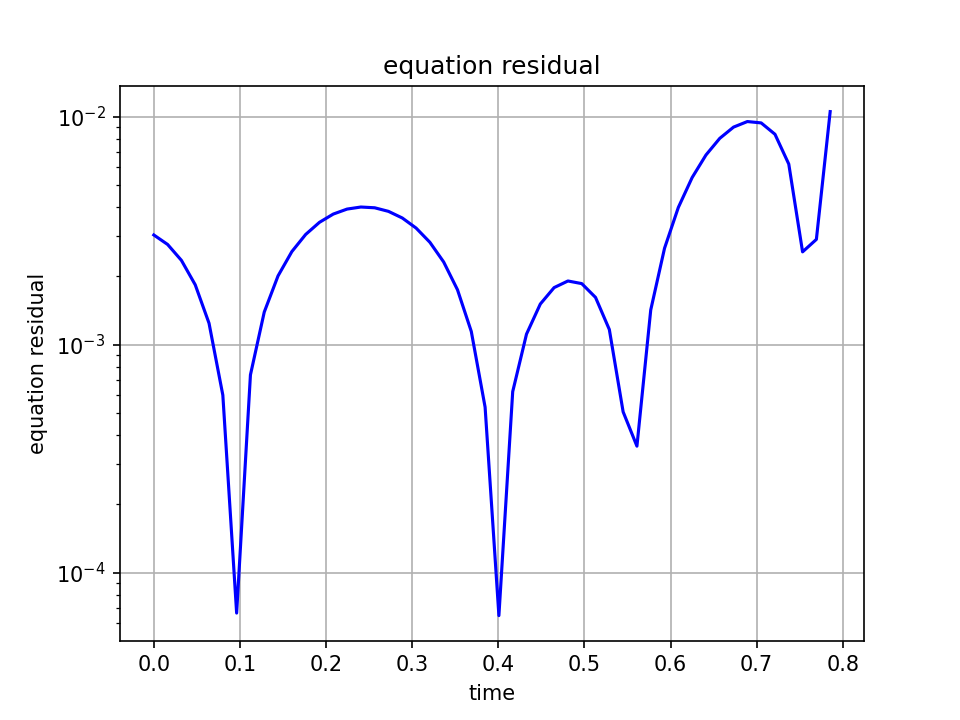
\includegraphics[scale = 0.5]{supportingFiles/residual.png}
	\caption{the residual of equation during prediction}
	\label{residualFig}
\end{figure}

\begin{figure}[!h]
	\centering
	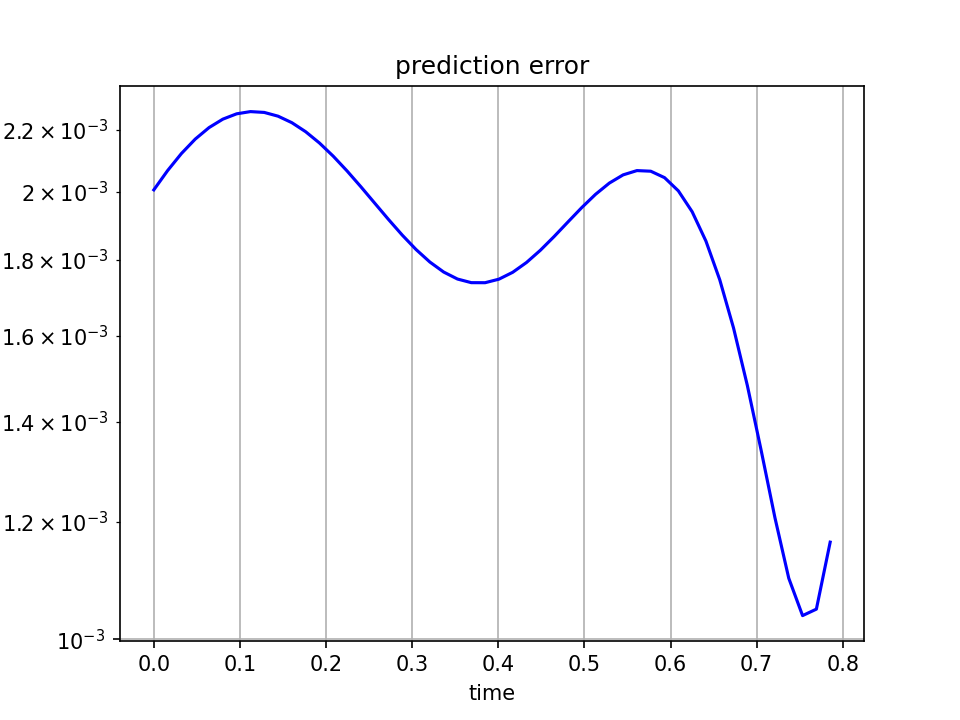
\includegraphics[scale = 0.5]{supportingFiles/error.png}
	\caption{error of predicted vs actual data}
	\label{errorFig}
\end{figure}

\begin{figure}[!h]
	\centering
	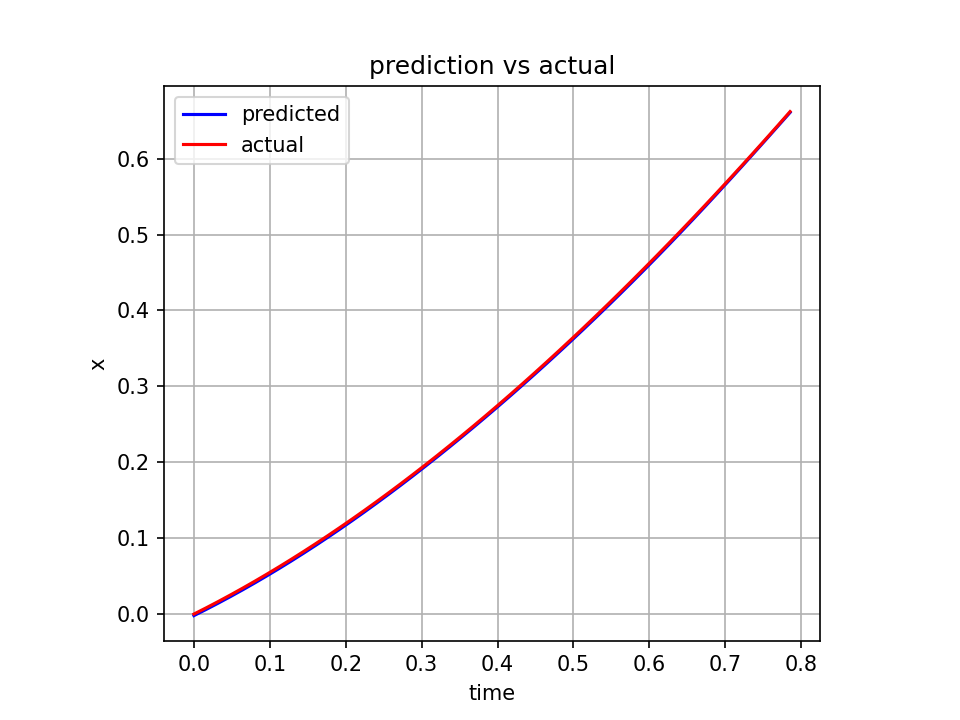
\includegraphics[scale = 0.5]{supportingFiles/output.png}
	\caption{predicted vs actual data comparison}
	\label{predvsactFig}
\end{figure}

The value of coefficient computed by the model is shown in \Cref{coeff_table} \\

\begin{table}
	\center
	\caption{predicted coefficient value}
	\begin{tabular}{|c|c|c|}
		\hline
		predicted value & actual value & error percentage \\ \hline \hline
		0.49910807 & 0.5 & 0.1783 \\ \hline
	\end{tabular}
	\label{coeff_table}
\end{table}

%------------------------------------------------------------------------------
\section{conclusion}
The present work shows that it is possible to do the parameter estimation
with limited dataset and the way to do optimization
with combined loss values. Hence, further works can be developed from this.

\center{*****}
\end{document}
